Speech technology is the basis for the creation of interfaces that allow a user to interact with machines using spoken language rather than with graphical display, keyboard, and mouse. Today these voice user interfaces (VUIs) are employed for partially or fully automating service offerings provided by companies to their customers, employees, or partners via telephone. Business domains that rely heavily on VUIs are banking, logistics, public transportation, and telecommunications. Other usages of Speech technology are interfaces to particular devices such as in-car navigation systems, and the employment of spoken language as an alternative to the input/output modalities of graphical user interfaces, e.g. in smartphones or tablets.

\begin{figure*}[htb]
  \colorrule{grey3}{\textwidth}{1.5pt}
  \center
  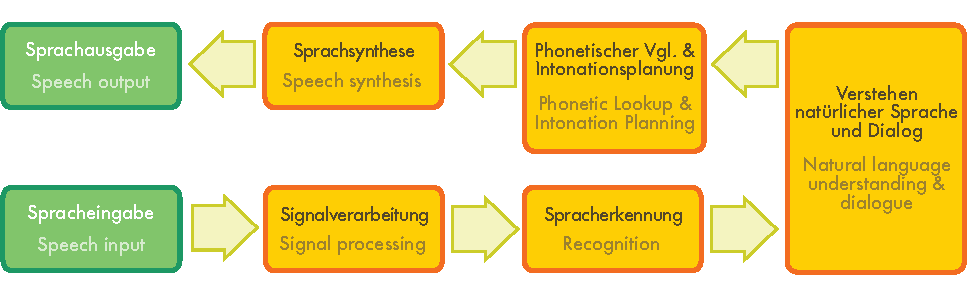
\includegraphics[width=\textwidth]{../_media/english/simple_speech-based_dialogue_architecture}
  \caption{Speech-based dialogue system}
  \label{fig:dialoguearch_en}
  \colorrule{grey3}{\textwidth}{1.5pt}
\end{figure*}

At its core, Speech technology comprises the following four different technologies:

\begin{enumerate}
\item Automatic \underbar{speech recognition} (ASR) is responsible for determining which words were actually spoken given a sequence of sounds uttered by a user.
\item \underbar{Syntactic analysis} and \underbar{semantic interpretation} deal with analysing the syntactic structure of a user’s utterance and interpreting the latter according to the purpose of the respective system.
\item \underbar{Dialogue management} is required for determining, on the part of the system the user interacts with, which action shall be taken given the user’s input and the functionality of the system.
\item \underbar{Speech synthesis} (Text-to-Speech, TTS) technology is employed for transforming the wording of that utterance into  sounds that will be output to the user. 
\end{enumerate}

One of the major challenges is to have an ASR system recognising the words uttered by a user as precisely as possible. This requires either a restriction of the range of possible user utterances to a limited set of keywords, or the manual creation of language models that cover a large range of natural language user utterances. A fundamental requirement for good performance is also a well trained acoustic model based on a huge amount of recorded data covering different accents, age groups, genders etc. Whereas the former results in a rather rigid and inflexible usage of a VUI and possibly causes a poor user acceptance, the creation, tuning and maintenance of acoustic and language models may increase the costs significantly. However, VUIs that employ language models and initially allow a user to flexibly express their intent – evoked by a ‘How may I help you’ greeting – show both a higher automation rate and higher user acceptance and may therefore be considered as advantageous over a less flexibly directed dialogue approach. An exception to the above mentioned are  so-called embedded systems. They require a  small set of commands and the usage of language models in such cases is a disadvantage. Embedded systems are today still successfully built with grammars. 

For the output part of a VUI, companies tend to use pre-recorded utterances of professional – ideally corporate – speakers a lot. Static utterances in which the wording does not depend on the particular contexts of use or the personal data of the given users will result in a rich user experience. However, the more dynamic the content an utterance needs to consider, the more the user experience may suffer from a poor prosody resulting from concatenating single audio files. In contrast, today’s TTS systems prove superior, though optimizable, regarding the prosodic naturalness of dynamic utterances.  

Regarding the market for Speech technology, the last decade underwent a strong standardisation of the interfaces between the different technology components, as well as by standards for creating particular software artefacts for a given application. There also has been strong market consolidation in the last ten years, particularly in the field of ASR and TTS. Here, the national markets in the G20 countries – i.e. economically strong countries with a considerable population - are dominated by few big players worldwide led mainly by Nuance, Google and Microsoft. 

Speech recognition in Slovakia has a long history but has been done only at universities or scientific institutions. Most places focus on basic research and solutions of specific problems of speech recognition. The Department of Speech Analysis and Synthesis of the Institute of Informatics of the Slovak Academy of Sciences as a participant of the SpeechDat-E project focuses mainly on acoustic models for telephony systems. With a growing number of speech data such as for example parliamentary discussions the institute is using existing tools for speech recognition to try to create widely usable acoustic models for applications such as dictation, talk transcription, etc. with focus on speaker dependent systems. The main focus of the Department of Telecommunication of the Slovak Technical University in Bratislava is the processing of speech signals in noisy conditions (speech/silence detection, features extraction, etc.). Among others, the department created several small speech recognition systems to compare the performance and usability of different free speech recognition systems for the Slovak language. At the Technical University of Košice there are several departments focusing on automatic speech recognition. The Department of Electronics and Multimedia Communications, which was originally focused mainly on basic research for the digital processing of speech signals, has gradually extended its research focus toward developing complex interactive speech systems. A few years ago in cooperation with research teams from the Slovak Academy of Sciences, Slovak University of Technology and University of Žilina the Smart Speech Communication System was developed at the Department of Electronics and Multimedia Communications. The system is available to public and continually serves as a demonstrator of the speech interactive services in Slovak over the telephone. Today one of the most noticeable outputs represents the activities in the field of language modelling for the Slovak large vocabulary continuous speech recognition system. The language model created at the department is based on a corpus of $2\cdot 10^9$ tokens. 
\newline The second important workplace at the Technical University of Košice is the Department of Cybernetics and Artificial Intelligence where the first voice retrieval information dialogue system and SAMPA for the Slovak language were created. Today the speech recognition activities at the department plays a rather minor role. The Department of Applied Mathematics and Statistics of the Faculty of Mathematics, Physics and Informatics at Comenius University in Bratislava is working mainly on speech recognition of isolated words for children's voices. The results were applied in an educational process to verify a text read by children. From the audio data recorded for the acoustic model training two speech databases have been created (\emph{Alica} and \emph{Viktória}).  The main institution for speech recognition at the University of Žilina is the Department of Telecommunications and Multimedia. Its team focuses mainly on digital signal processing for speech recognition and recognition of isolated words using Hidden Markov Models.

Close cooperation between the Department of Electronics and Multimedia Communications of the Technical University of Košice and the Department of Speech Analysis and Synthesis of the Institute of Informatics of the Slovak Academy of Sciences resulted in the first visible success in developing the Slovak large vocabulary continuous speech recognition system. The result of the cooperation is an automatic speech dictation system commercially usable in judiciary.

Regarding commercial systems for Slovak speech recognition, it is worth mentioning the product from Newton Technology Company. It can be considered as the first usable speaker independent dictation system for the Slovak language.

Looking beyond today’s state of technology, there will be significant changes due to the spread of smartphones as a new platform for managing customer relationships – in addition to the telephone, internet, and email channels. This tendency will also affect the employment of technology for Speech Interaction. On one hand, demand for telephony-based VUIs will decrease in long run. On the other hand, the usage of spoken language as a user-friendly input modality for smartphones will gain significant importance. This tendency is supported by the observable improvement of speaker-independent speech recognition accuracy for speech dictation services that are already offered as centralised services to smartphone users. Given this ‘outsourcing’ of the recognition task to the infrastructure of applications, the application-specific employment of linguistic core technologies will supposedly gain importance compared to the present situation. 
